%*******************************************************************************
%*********************************** First Introduction *****************************
%*******************************************************************************
%\chapter{Introduction}  %Title of the First Introduction
%\chapter*{Introduction}
\chapter{Core}  %Title of the First Introduction
%\addcontentsline{tableofcontents}{chapter}{introduction}

\ifpdf
    \graphicspath{{Core/Figs/Raster/}{Core/Figs/PDF/}{Core/Figs/}}
\else
    \graphicspath{{Core/Figs/Vector/}{Core/Figs/}}
\fi

%********************************** %First Section  **************************************
\section{Data Collection} %Section - 1.1 
Our dataset is the Variome Corpus\cite{verspoor2013annotating}, which is openly accessible. \footnote{\href{http://www.opennicta.com.au/home/health/variome}\url{http://www.opennicta.com.au/home/health/variome}} \citet{verspoor2013annotating} gave a detailed illustration of the document selection and annotation process. I will summarize the main points here.
\subsection{Background}
A major part of the current biomedical research lies in understanding the relations between human genetic variation and disease phenotypes. The \emph{Human Variome Project}, or \emph{HVP}, is a global initiative to collect all genetic variation information affecting human health\cite{ring2006human}. In particular, it acts as a liaison between individuals and organizations to integrate the genetic variants into databases that are open to the general public\cite{verspoor2013annotating}. The \emph{International Society for Gastrointestinal Hereditary Tumours (InSiGHT)}, is an international organization which aims to benefit patients with hereditary gastrointestinal(GI) tumours by research, education and personal assistance. In 2008, InSiGHT and HVP began a collaboration which propels InSiGHT to refine its process in the integration and interpretation of genetic variants. Consequently, a substantial effort was made to understand the mutation of mismatch repair(MMR) genes, the cause of Lynch Syndrome - one of the main syndromes of GI cancer\cite{silva2009mismatch}. A total of 10 full-text articles were selected from PubMed Central\textregistered  by searching the common Lynch syndrome genes. These documents are mostly about inherited colon cancer. The annotation schema, also known as the Variome Annotation Schema\cite{verspoor2013annotating}, include 11 entity types and 13 relation types. as can be seen in the table here
\begin{table}
	\caption{A nice looking table}
	\centering
	\label{table:nice_table}
	\begin{tabular}{l c c c c}
		\hline 
		\multirow{2}{*}{Dental measurement} & \multicolumn{2}{c}{Species I} & \multicolumn{2}{c}{Species II} \\ 
		\cline{2-5}
		& mean & SD  & mean & SD  \\ 
		\hline
		I1MD & 6.23 & 0.91 & 5.2  & 0.7  \\
		
		I1LL & 7.48 & 0.56 & 8.7  & 0.71 \\
		
		I2MD & 3.99 & 0.63 & 4.22 & 0.54 \\
		
		I2LL & 6.81 & 0.02 & 6.66 & 0.01 \\
		
		CMD & 13.47 & 0.09 & 10.55 & 0.05 \\
		
		CBL & 11.88 & 0.05 & 13.11 & 0.04\\ 
		\hline 
	\end{tabular}
\end{table}

In short, the corpus is Inspired by needs of inSIGHT database, but intended for broader applications. Documents relevant to the genetics of Lynch syndrome, which covers inherited colon cancer as well as certain other cancers. Selected with PubMed Central To train tools for mining genetic variation and its relationship to disease
Here in this information extraction task, we treat the manually annotated data as the \emph{gold data}, 
\section{Dependency Graph and Shortest Path}
	\begin{figure}
		\centering
			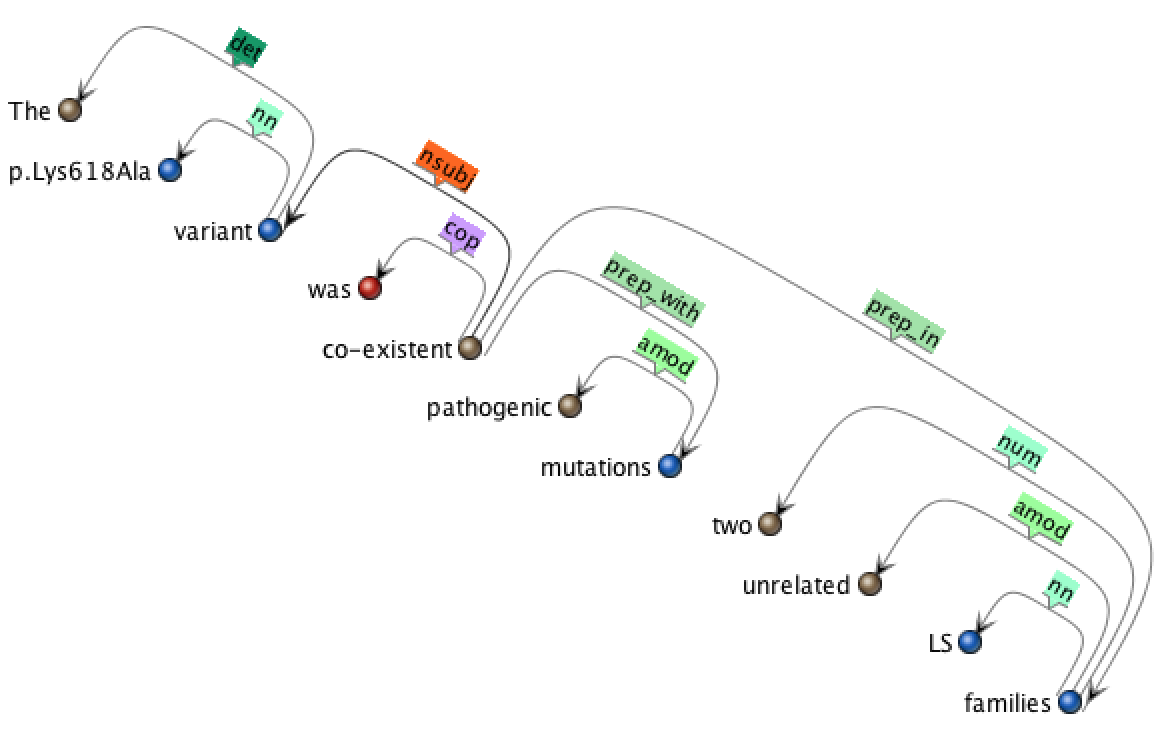
\includegraphics[width=\textwidth]{Dependency_Graph}
			\caption{Dependency Graph}
			\label{fig:Dependency_Graph}   
	\end{figure}

The dependency graph of a sentence is a directed graph, where nodes represent sentence tokens, and edges indicate their semantic relations. Figure \ref{fig:Dependency_Graph} shows the dependency graph of the sentence \emph{`` The p.Lys618Ala variant was co-existent with pathogenic mutations in two unrelated LS families.''} generated by the Stanford Parser. Such a graph preserves the rich semantic structure of a sentence, and has been widely regarded as an informative way of presenting a sentence. A detailed explanation of the relative constituents in the graph can be found in \cite{de2008stanford}. However, the point is to transfer only human-readable sentences to a computer-understandable data structure. The general idea would be to feed this graph into a learning algorithm and classify relations based on similarity to the sentence graph in the training set. Different approaches exist for this process. Turku Event Extraction System (TEES)\footnote{https://github.com/jbjorne/TEES}, for instance, engineers a feature vector which consists of token features(part-of-speech tags and character constituents for each word), sentence features(bag-of-words counts), and graph-based features(dependency path represented as N-grams) and builds a SVM model with the feature vector\cite{bjorne2011generalizing}. In this project, we decide to use the \emph{Shortest Path Hypothesis}\cite{bunescu2005shortest}, namely the heuristic that the relation between two entities in a sentence can be distilled from the shortest path between these entities in the undirected version of the sentence dependency graph. This effectively reduces the burden of feature engineering\cite{liu2013approximate}, but it also calls for high-quality training data. We believe that with effective parameter tuning and clever graph matching techniques, the shortest path can be a single standalone feature for a relation between two entities.
\section{Approximate Subgraph Matching Algorithm}



To separate Named Entity Recognition from Relation Extraction problem, the named entity annotations are provided in training, development and test sets. Effectively, this is just asking computer to extract possible relations between these entities without worrying how to recognize them accurately. Of course, named entity recognition is an important step in a real relation extraction task as cite cite, because biological named entity recognition is such a complex problem and sometimes the relation extraction success would depend on the accuracy of NER.

the performance of the subgraph matching method, as an instance-based learning strategy (Alpaydin, 2004), is dependent on having good training examples that express the events in a range of syntactic structures, cite





\section{System Adaptation}
As mentioned in \ref{section1.3}, the project aims at adapting an existing system used for event-retrieval tasks on relation extraction tasks.
\subsection{BioNLP Shared Tasks}
BioNLP shared Task series is a community-wide text mining challenge specifically for biomedical literatures. The GE task in shared task 2013 aims at retireving events of the following format:
\begin{table}
	\caption{Events}
	\centering
	\label{table:events}
	\begin{tabular}{l c c c c}
		\hline 
		\multirow{2}{*}{Dental measurement} & \multicolumn{2}{c}{Species I} & \multicolumn{2}{c}{Species II} \\ 
		\cline{2-5}
		& mean & SD  & mean & SD  \\ 
		\hline
		I1MD & 6.23 & 0.91 & 5.2  & 0.7  \\
		
		I1LL & 7.48 & 0.56 & 8.7  & 0.71 \\
		
		I2MD & 3.99 & 0.63 & 4.22 & 0.54 \\
		
		I2LL & 6.81 & 0.02 & 6.66 & 0.01 \\
		
		CMD & 13.47 & 0.09 & 10.55 & 0.05 \\
		
		CBL & 11.88 & 0.05 & 13.11 & 0.04\\ 
		\hline 
	\end{tabular}
\end{table}

The a1 files does (to be added), the a2 files does (to be added), 

\subsection{Variome Annotation Schema}
\begin{table}
	\caption{Relations under Variome Annotation Schema}
	\centering
	\label{table:relations}
	\begin{tabular}{l c c c c}
		\hline 
		\multirow{2}{*}{Dental measurement} & \multicolumn{2}{c}{Species I} & \multicolumn{2}{c}{Species II} \\ 
		\cline{2-5}
		& mean & SD  & mean & SD  \\ 
		\hline
		I1MD & 6.23 & 0.91 & 5.2  & 0.7  \\
		
		I1LL & 7.48 & 0.56 & 8.7  & 0.71 \\
		
		I2MD & 3.99 & 0.63 & 4.22 & 0.54 \\
		
		I2LL & 6.81 & 0.02 & 6.66 & 0.01 \\
		
		CMD & 13.47 & 0.09 & 10.55 & 0.05 \\
		
		CBL & 11.88 & 0.05 & 13.11 & 0.04\\ 
		\hline 
	\end{tabular}
\end{table}

During the duration of this project, most of my attempts to fully adapt the system to relation extraction tasks have failed. In essence, the differentiation in the retrieval process lies in the event retrieval relies on the detection and prediction of a trigger word, where as the relation extraction does not. 

\section{Results}

